\documentclass[12pt]{amsart}
\usepackage[utf8]{inputenc}


\makeatletter
\def\specialsection{\@startsection{section}{1}%
  \z@{\linespacing\@plus\linespacing}{.5\linespacing}%
%  {\normalfont\centering}}% DELETED
  {\normalfont}}% NEW
\def\section{\@startsection{section}{1}%
  \z@{.7\linespacing\@plus\linespacing}{.5\linespacing}%
%  {\normalfont\scshape\centering}}% DELETED
  {\normalfont\scshape}}% NEW
\makeatother

\makeatletter
\def\@tocline#1#2#3#4#5#6#7{\relax
  \ifnum #1>\c@tocdepth % then omit
  \else
    \par \addpenalty\@secpenalty\addvspace{#2}%
    \begingroup \hyphenpenalty\@M
    \@ifempty{#4}{%
      \@tempdima\csname r@tocindent\number#1\endcsname\relax
    }{%
      \@tempdima#4\relax
    }%
    \parindent\z@ \leftskip#3\relax \advance\leftskip\@tempdima\relax
    \rightskip\@pnumwidth plus4em \parfillskip-\@pnumwidth
    #5\leavevmode\hskip-\@tempdima
      \ifcase #1
       \or\or \hskip 1em \or \hskip 2em \else \hskip 3em \fi%
      #6\nobreak\relax
    \dotfill\hbox to\@pnumwidth{\@tocpagenum{#7}}\par
    \nobreak
    \endgroup
  \fi}
\makeatother
%\usepackage{hyperref}

\addtolength{\hoffset}{-2.25cm}
\addtolength{\textwidth}{4.5cm}
\addtolength{\voffset}{-2.5cm}
\addtolength{\textheight}{5cm}
\setlength{\parskip}{0pt}
\setlength{\parindent}{15pt}

\usepackage{amsmath , amssymb , amsthm}
\makeatletter
\renewcommand*\env@matrix[1][*\c@MaxMatrixCols c]{%
  \hskip -\arraycolsep
  \let\@ifnextchar\new@ifnextchar
  \array{#1}}
\makeatother
\usepackage[colorlinks = true, linkcolor = black, citecolor = black, final]{hyperref}
\usepackage{graphicx}
\usepackage{multicol}
\usepackage{ marvosym }
\usepackage{wasysym}
\usepackage{tikz}
%\usepackage{amsmath}
\usepackage{fancyhdr}
\usepackage{romannum}
\usepackage{mathtools}
\usepackage{listings}
\usepackage{xcolor}
\usepackage{tcolorbox}
\tcbuselibrary{minted,breakable,xparse,skins}
\usepackage{caption}

\definecolor{bg}{gray}{0.95}
\DeclareTCBListing{mintedbox}{O{}m!O{}}{%
  breakable=true,
  listing engine=minted,
  listing only,
  minted language=#2,
  minted style=default,
  minted options={%
    linenos,
    gobble=0,
    breaklines=true,
    breakafter=,,
    fontsize=\small,
    numbersep=8pt,
    #1},
  boxsep=0pt,
  left skip=0pt,
  right skip=0pt,
  left=25pt,
  right=0pt,
  top=3pt,
  bottom=3pt,
  arc=5pt,
  leftrule=0pt,
  rightrule=0pt,
  bottomrule=2pt,
  toprule=2pt,
  colback=bg,
  colframe=white!70,
  enhanced,
  overlay={%
    \begin{tcbclipinterior}
    \fill[gray!20!white] (frame.south west) rectangle ([xshift=20pt]frame.north west);
    \end{tcbclipinterior}},
  #3}
%\usepackage{pythonhighlight}
\usepackage{minted}


\usemintedstyle{borland}
\usepackage{pythonhighlight}
\usetikzlibrary{patterns}
\newcommand{\ds}{\displaystyle}
\DeclareMathOperator{\sech}{sech}
\setlength{\parindent}{0in}
\pagestyle{plain}

%\pagestyle{empty}
\usemintedstyle{borland}
\newcommand\norm[1]{\left\lVert#1\right\rVert}

\renewcommand{\contentsname}{Table of Contents}




\begin{document}

\begin{titlepage}
   \begin{center}
       \vspace*{1cm}

       \textbf{Computational Neuroscience}

       \vspace{0.7cm}
        \textbf{EEE 482/582}
            
       \vspace{0.7cm}

       \textbf{Can Kocagil} 
       
       \vspace{0.7cm}
       \textbf{21602218}

       %\vfill
       \vspace{0.7cm}
            
       \textbf{Homework-1}
            
       \vspace{0.8cm}
         \begin{figure}[h]
            \centering
            
\includegraphics[width = 0.35\textwidth]{images/bilkent_logo.png}
            %\caption{}
            %\label{fig:mesh1}
        \end{figure}
      % 
\includegraphics[width=0.4\textwidth]{images/bilkent_logo.png}
       \vspace{0.7cm}  
       Department of Electric \& Electronics Engineering \\
       \vspace{0.7cm}
       Bilkent University\\
       \vspace{0.7cm}
       Ankara, Turkey \\
       \vspace{0.7cm}
       5.02.2021
            
   \end{center}
\end{titlepage}

\tableofcontents
\listoffigures
\listoftables
\lstlistoflistings

\newpage

%\thispagestyle{empty}

{\scshape EEE 482} \hfill {\scshape \large  Homework-\romannumeral1\relax} \hfill {\scshape Can Kocagil}
\smallskip
\hrule


\pagenumbering{arabic}

\section{Question 1}

In this question, we assume that neural population computes weighted linear combination of its input $x$ that is characterized by a linear system of the following equation
\begin{align*}
 Ax = b \text{ where A is the transfer function and b is the output vector} 
\end{align*}

Then, the single output measurement is given by

\[
\begin{pmatrix}
 1 & 0& -1& 2\\ 
 2&  1& -1& 5\\ 
 3&  3& 0& 9
\end{pmatrix}
\begin{pmatrix}
 x_{1}  \\ 
 x_{2}  \\ 
 x_{3}  \\
 x_{4}
\end{pmatrix} =
\begin{pmatrix}
0 \\
0 \\
0 
\end{pmatrix}
\]

\subsection{Part A}

In part a, we are asked to find all solutions such that $x_n$ satisfies the equation $Ax_n = 0$. In other means, we need to find the homogeneous solution to the system of $Ax_n = 0$. Hence, to find a homogeneous solution for this system, we should firstly apply Gauss – Jordan elimination by elementary row equations to obtain row echelon form of the given matrix. To do that, we can proceed by the following steps 

\[
\begin{pmatrix}
 1 & 0& -1& 2\\ 
 2&  1& -1& 5\\ 
 3&  3& 0& 9
\end{pmatrix} \overset{r_3 \leftarrow r_1+r_2}{\longrightarrow} 
\begin{pmatrix}
 1 & 0& -1& 2\\ 
 2&  1& -1& 5\\ 
 0&  3& 3& 3
\end{pmatrix}  \overset{r_2 \leftarrow r_2-2r_1}{\longrightarrow} 
\begin{pmatrix}
  1 & 0& -1& 2\\ 
 0&  1& 1& 1\\ 
 0&  3& 3& 3
\end{pmatrix} \overset{r_3 \leftarrow r_3-3r_2}{\longrightarrow} 
\begin{pmatrix}
 1 & 0& -1& 2\\ 
 0&  1& 1& 1\\ 
 0&  0& 0& 0
\end{pmatrix}
\]

Hence, we successfully obtain the row echelon for of $A$, such that we have
\[
\begin{pmatrix}
 1 & 0& -1& 2\\ 
 0&  1& 1& 1\\ 
 0&  0& 0& 0
\end{pmatrix}
\begin{pmatrix}
 x_{1}  \\ 
 x_{2}  \\ 
 x_{3}  \\
 x_{4}
\end{pmatrix} = 
\begin{pmatrix}
1 \\
4 \\
9 
\end{pmatrix}
\]

Note that the Gauss–Jordan elimination does not affect the solutions $x_n$ of the linear system. Then, we can observe that $x_1$  and $x_2$ are the pivot variables. From that, we can inference that $x_3$ and $x_4$ are free variables that means that the solution can be written in terms of any value of $x_3$ and $x_4$.  Actually, this is kind of result is expected because the number of equations is less than the number of unknowns. Also, note that the matrix A can be called rank deficient matrix. Therefore, then we can parametrize the $x_3$ and $x_4$ as a following way

\begin{equation*}
  x_3 = \alpha  \text{ and } x_4 = \beta \text{ where } \alpha \text{ and } \beta \in \mathbb{R}  
\end{equation*}


From the equations
\[
\begin{matrix}
x_{1} - x_{3} + 2x_{4} = 0\\
x_{2} + x_{3} + x_{4}  = 0
\end{matrix} \Longrightarrow
\begin{matrix}
x_{1} = x_{3} - 2x_{4} \\
x_{2} = -x_{3} - x_{4} 
\end{matrix}
\]

the solution $x_n$  to the homogeneous system $Ax_n = 0$ can be written as the following way

\[
x_n = \begin{pmatrix}
 \alpha - 2\beta\\ 
 \alpha - \beta\\ 
 \alpha \\
 \beta
\end{pmatrix} = \alpha
\begin{pmatrix}
 1\\ 
 -1\\ 
 1 \\
 0
\end{pmatrix} + 
\begin{pmatrix}
 -2\\ 
 -1\\ 
 0\\
 1
\end{pmatrix}
\forall \alpha , \beta \in \mathbb{R}
\]\\


%\underset{\overset{r_1-4r_2}{\longrightarrow}}{\overset{r_1+r_2}{\longrightarrow}}
Then, we need to verify the hand driven answer by using computer. To do that, I utilize Python’s standard numerical computation framework NumPy. Here is the verification Python code.
\newpage
{\scshape EEE 482} \hfill {\scshape \large  Homework-\romannumeral1\relax} \hfill {\scshape Can Kocagil}
\smallskip
\hrule

\begin{mintedbox}{python}
import numpy as np
    
# Let's create the matrix A :
A = np.array([[1, 0, -1, 2],
              [2, 1, -1, 5],
              [3, 3, 0, 9]])

# Since alpha ve beta are arbitrary scalars:
alpha, beta = (np.random.randn() , np.random.randn())

# Hand driven solution to the system of Ax = 0, x_n is:
x_n = np.array([[alpha - 2 * beta],
               [-alpha - beta],
               [alpha],
               [beta]])

# Verification of the solution x_n to the system A * x_n = 0 :
print(f"Proof that x_n solves the linear system of Ax = 0 is \n {A @ x_n} \n")
Q1_TEST = lambda x_n : np.isclose(np.zeros((3,1)), A @ x_n)
print(f'Q1 Verification \n {Q1_TEST(x_n)}')
\end{mintedbox}

\iffalse
\begin{minted}
[
frame=lines,
framesep=2mm,
baselinestretch=1.2,
fontsize=\footnotesize,
linenos
]
{python}
import numpy as np
    
# Let's create the matrix A :
A = np.array([[1, 0, -1, 2],
              [2, 1, -1, 5],
              [3, 3, 0, 9]])

# Since alpha ve beta are arbitrary scalars:
alpha, beta = (np.random.randn() , np.random.randn())

# Hand driven solution to the system of Ax = 0, x_n is:
x_n = np.array([[alpha - 2 * beta],
               [-alpha - beta],
               [alpha],
               [beta]])

# Verification of the solution x_n to the system A * x_n = 0 :
print(f"Proof that x_n solves the linear system of Ax = 0 is \n {A @ x_n} \n")
Q1_TEST = lambda x_n : np.isclose(np.zeros((3,1)), A @ x_n)
print(f'Q1 Verification \n {Q1_TEST(x_n)}')


\end{minted}
\fi


Output:

Proof that $x_n$ solves the linear system of $Ax = b$ is \\
\text{[[0.00000000e+00] 
[0.00000000e+00]
[1.77635684e-15]] }  
\\
Q1 Verification  \\
\text{[[ True]  [ True]  [ True]] } 

\subsection{Part B}
In this part of the question, we are asked to find a particular solution to $x_p$ such that $Ax_p  = b$. As done in the part a, we should perform elementary row operations to find a particular solution $x_p$ that solves the given system. However, in this case, we should augment the matrix with the given vector b such that we have a form of concatenated matrix with the following structure
\[ 
\begin{pmatrix}[c|c]
  A & b\\
\end{pmatrix} = 
\begin{pmatrix}[cccc|c]
  1 & 0 & -1& 2& 1\\
  2 & 1 & -1& 5& 4 \\
  3 & 3 & 0& 2& 9 \\
\end{pmatrix}
\]

Then, again by applying elementary row operations we have 

\[
\begin{pmatrix}[cccc|c]
  1 & 0 & -1& 2& 1\\
  2 & 1 & -1& 5& 4 \\
  3 & 3 & 0& 2& 9 \\
\end{pmatrix}\overset{r_2 \leftarrow r_2-2r_1} {\longrightarrow} 
\begin{pmatrix}[cccc|c]
 1 & 0& -1& 2& 1 \\ 
 0&  1& 1& 1& 2\\ 
 3&  3& 0& 9& 9
\end{pmatrix}  \overset{r_3 \leftarrow r_1+r_2}{\longrightarrow} 
\begin{pmatrix}[cccc|c]
 1 & 0& -1& 2& 1 \\ 
 0&  1& 1& 1& 2\\ 
 0&  3& 3& 3& 6
\end{pmatrix} \overset{r_3 \leftarrow r_3-3r_2}{\longrightarrow} 
\begin{pmatrix}[cccc|c]
 1 & 0& -1& 2& 1\\ 
 0&  1& 1& 1& 2\\ 
 0&  0& 0& 0& 0
\end{pmatrix}
\]

Hence, we obtain the row echelon form of augmented matrix 
$
\begin{pmatrix}[c|c]
  A & b\\
\end{pmatrix}. 
$
Then, we can write the equation as a
\[
\begin{pmatrix}
 1 & 0& -1& 2\\ 
 0&  1& 1& 1\\ 
 0&  0& 0& 0
\end{pmatrix} 
\begin{pmatrix}
 x_{1}  \\ 
 x_{2}  \\ 
 x_{3}  \\
 x_{4}
\end{pmatrix} = 
\begin{pmatrix}
1 \\
2 \\
0
\end{pmatrix} where \hspace{2mm} rref(A) = 
\begin{pmatrix}
 1 & 0& -1& 2\\ 
 0&  1& 1& 1\\ 
 0&  0& 0& 0
\end{pmatrix} 
\]

\newpage
{\scshape EEE 482} \hfill {\scshape \large  Homework-\romannumeral1\relax} \hfill {\scshape Can Kocagil}
\smallskip
\hrule
\vspace{2mm}

By solving the following equations in LHS we obtain the expression in RHS

\[
\begin{matrix}
x_{1} - x_{3} + 2x_{4} = 1\\
x_{2} + x_{3} + x_{4}  = 2
\end{matrix} \Longrightarrow
\begin{matrix}
x_{1} = x_{3} - 2x_{4} + 1\\
x_{2} = -x_{3} - x_{4} + 2
\end{matrix}
\]



From the above equations, we can select the x vector values  as a $x_1 = 1 , x_2 = 2, x_3 = 0$ and $x_4$ = 0 so that 

\begin{center}
    $x_p$ = $\begin{pmatrix}
 x_{1}  \\ 
 x_{2}  \\ 
 x_{3}  \\
 x_{4}
\end{pmatrix}$ = 
$\begin{pmatrix}
 1  \\ 
 2  \\ 
 0  \\
 0
\end{pmatrix}$ and solves the
$\begin{pmatrix}
 1 & 0& -1& 2\\ 
 0&  1& 1& 1\\ 
 0&  0& 0& 0
\end{pmatrix}$ $x_p$ = 
$\begin{pmatrix}
 1  \\ 
 2  \\ 
 0 
\end{pmatrix}$

\end{center}
 
Then, let’s verify our results using Python. Here is the python code for verification of part b.   


\begin{mintedbox}{python}
# Let's create the matrix A :
A = np.array([[1, 0, -1, 2],
              [2, 1, -1, 5],
              [3, 3, 0, 9]])

# Let's create output vector b :
b = np.array([[1],
              [4],
              [9]])

# Particular solution to the system A * x_p = b :
x_p = np.array([[1],
               [2],
               [0],
               [0]])
# Verification of the solution x_n to the system A * x_p = 0 :
print(f"Proof that x_p solves the linear system of Ax = b is \n {A @ x_p} \n")
Q1_TEST = lambda x_p : np.isclose(b, A @ x_p)
print(f'Q1 Verification \n {Q1_TEST(x_p)}')

\end{mintedbox}

Proof that $x_p$ solves the linear system of $Ax = b$ is 
 [[1]
 [4]
 [9]] 

Q1 Verification 
 [[ True]
 [ True]
 [ True]]

\subsection{Part C}
Adopting the solution obtained in part b, we can generalize the solution by equating the free variables $x_3$  and $x_4$ as $\alpha$ and $\beta$  where $\alpha$ and $\beta$ $\in$ $\mathbb{R}$, respectively. Then, let $\xi$ be the generalized version of the solution set that equals to \\

%\xi = 
\begin{equation*}
\hspace{2mm} \xi =
\begin{pmatrix}
 \alpha - 2\beta + 1\\ 
 \alpha - \beta + 2\\ 
 \alpha \\
 \beta
\end{pmatrix} = \alpha
\begin{pmatrix}
 1\\ 
 -1\\ 
 1 \\
 0
\end{pmatrix} + \beta 
\begin{pmatrix}
 -2\\ 
 -1\\ 
 0\\
 1
\end{pmatrix} + 
\begin{pmatrix}
 1\\ 
 2\\ 
 1 \\
 0
\end{pmatrix} \hspace{2mm} \forall \alpha, \beta \in \mathbb{R} \hspace{2mm} \text{where} \hspace{2mm} x_3 = \alpha \hspace{2mm}  \text{and}  \hspace{2mm} x_4 = \beta
\end{equation*}


Then, we can take any arbitrary scalar for $\alpha$ and $\beta$, and let $x_{general}$ be the any vector taken from the solution set $\xi$. The following Python code proves that $x_{general}$ is a valid solution to the system  $Ax_{general}  = b$.

\newpage
{\scshape EEE 482} \hfill {\scshape \large  Homework-\romannumeral1\relax} \hfill {\scshape Can Kocagil}
\smallskip
\hrule
\vspace{2mm}



\begin{mintedbox}{python}
# Let's create the matrix A :
A = np.array([[1, 0, -1, 2],
              [2, 1, -1, 5],
              [3, 3, 0, 9]])

# Since alpha ve beta are arbitrary scalars:
alpha, beta = (np.random.randn() , np.random.randn())

# Hand driven solution to the system of Ax = b, x_general is:
x_general = np.array([[alpha - 2 * beta + 1],
                      [-alpha - beta + 2],
                      [alpha],
                      [beta]])
# Verification of the solution x_general to the system A * x_general = b :
print(f"Proof that x_general solves the linear system of Ax = b is \n {A @ x_general} \n")
Q1_TEST = lambda x_general : np.isclose(b, A @ x_general)
print(f'Q1 Verification \n {Q1_TEST(x_general)}')


\end{mintedbox}

Proof that $x_{general}$ solves the linear system of $Ax = b$ is 
 [[1.]
 [4.]
 [9.]] 

Q1 Verification 
 [[ True]
 [ True]
 [ True]]

\subsection{Part D}

In this part, we are asked to find pseudo-inverse of $A$ that can be denoted by $A^+$. In the context of linear algebra, pseudo inverse (Say $A^+$) is the generalized version of inverse matrix (Say $A^{-1}$). To give brief information on the context, the general approach for using pseudo-inverse is to find least squared solution to a linear system. Moreover, the main advantage of the pseudo-inverse is that it does not have strict constraint about being square matrix so it can be applied on any matrix. Then, to compute the  $A^+$, the prior step is to find Singular Value Decomposition (SVD) of $A$ since our matrix $A$ is rank deficient. The following equation describes the SVD of $A$ and relationship between the $A^+$

\begin{equation}
    \text{Let} \hspace{2mm} A_{mxn} = U_{mxm}  \Sigma_{mxn}  V^T_{mxn}  \hspace{2mm} \text{so that} \hspace{2mm} A^{+} = V \Sigma_{}^+ U^T
\end{equation}

Where $U$ is the $m$x$m$ orthonormal matrix such that the columns of $U_{mxm}$ is called “left singular vectors” of $A$, $\Sigma_{mxn}$ is a diagonal matrix holds singular values diagonally and $V_{nxn}^T$ is orthonormal matrix whose columns are called “right singular vectors” of $A$. The problem statement of computing right singular values can be rewritten in the following eigen-value format
\begin{equation}
    A^T A v = \sigma^2v \hspace{2mm} \text{such that} \hspace{2mm} v \neq  0 \text{ and where $\sigma$ is a singular value} 
\end{equation}

In the same fashion, the left singular values can be computed the following eigen-value problem statement
\begin{equation}
    AA^T u = \sigma^2u \hspace{2mm} \text{such that} \hspace{2mm} u \neq  0 \text{ and where $\sigma$ is a singular value} 
\end{equation}

Therefore, we have 2 eigen-value problem statement. In other means, to find the term $\sigma^2$, we should solve the problem as it is eigen-value problem. From the equations (2) and (3), we can conclude that $AA^T$ and $A^TA$ share the same eigen values $\sigma^2$. Utilizing the term  $\sigma^2$ is exists in both equations, we need to compute both  $AA^T$ and $A^TA$ to obtain expressions for left and right singular vectors and values, respectively. By matrix multiplication, we have
\newpage
{\scshape EEE 482} \hfill {\scshape \large  Homework-\romannumeral1\relax} \hfill {\scshape Can Kocagil}
\smallskip
\hrule
\vspace{2mm}
\[ A^TA =
\begin{pmatrix}
  14 & 11 & -3& 39\\
  11 & 10 & -1& 32\\
  -3 &-1 & 2& 7 \\
  39& 32& -1& 110
\end{pmatrix} \text{and}\hspace{2mm}
AA^T =
\begin{pmatrix}
  6 & 13 & 21\\
  13 & 31 & 54\\
  -21 & 54 & 99 
\end{pmatrix}
\]


Back to eigen-value problem statements, we have

\begin{equation}
\begin{matrix}
(A^TA - I_4 \sigma^2)v = 0\\
(AA^T - I_3 \sigma^2)u = 0
\end{matrix} \Longrightarrow
\begin{matrix}
det(A^TA - I_4 \sigma^2) = 0\\
det(AA^T - I_3 \sigma^2) = 0
\end{matrix}
\end{equation}

By letting $\lambda$ = $\sigma^2$, we can compute singular values as a

\[
\begin{vmatrix}
6 - \lambda & 13 & 21\\
13 & 31-\lambda & 54 \\
21 & 54& 99-\lambda
\end{vmatrix} = -\lambda^3 + 136\lambda^2 - 323\lambda \Longrightarrow \lambda_{1,2,3} = \sigma^2_{1,2,3} = 0, 68 \pm \sqrt{4301}
\]

Since, the analytic derivations of the following steps are bit complex to derive by hand, I run the same procedure in Python. Before that, note that the definition of pseudo-inverse state that the matrix multiplication of $A$ with $A^+$ followed by $A$ equals to $A$. The mathematical expression for that

\begin{equation}
    AA^+ = A
\end{equation}


Then, let’s compute pseudo-inverse in Python

\begin{mintedbox}{python}
# Let's apply SVD on matrix A :
U, S, V_T = np.linalg.svd(A)

# Little bit of calculation :
(m,n) = A.shape
S_plus = np.zeros((m,n))
S_plus[:m, :m] = np.diag(np.concatenate((1 / S[:2], np.array([0]))))

print(f"Pseudo-inverse of A, A_plus is \n {V_T.T @ S_plus.T @ U.T} ")

Q1_TEST = lambda S_plus : np.isclose( np.linalg.pinv(A), V_T.T @ S_plus.T @ U.T)
print(f'Q1 Verification \n {Q1_TEST(S_plus)}')

print(f"Pseudo-inverse of A, A_plus by pinv() method is \n {np.linalg.pinv(A)} ")

\end{mintedbox}


Pseudo-inverse of A,A\_plus is \newline
 [[ 0.12693498  0.10835913 -0.05572755]  \newline
 [-0.23529412 -0.17647059  0.17647059]   \newline
 [ 0.01857585  0.04024768  0.06501548]] 

Q1 Verification \newline
 [[ True  True  True] \newline
 [ True  True  True]  \newline
 [ True  True  True]  \newline
 [ True  True  True]] 



 
\newpage
{\scshape EEE 482} \hfill {\scshape \large  Homework-\romannumeral1\relax} \hfill {\scshape Can Kocagil}
\smallskip
\hrule
\vspace{2mm}

Pseudo-inverse of A, $A_{plus}$ by pinv() method is \newline
 [[ 0.12693498  0.10835913 -0.05572755] \newline
 [-0.23529412 -0.17647059  0.17647059] \newline
 [-0.3622291  -0.28482972  0.23219814]  \newline
 [ 0.01857585  0.04024768  0.06501548]]


Note that little bit of computation is done to stabilize the numerical instability. The results between self-written pseudo-inverse and NumPy pinv() method is exactly same. Hence, we successfully compute the pseudo-inverse of A. \\

\subsection{Part E}
In this part of the question, the aim is to find sparsest solution to the system $Ax  = b$. In other means, we need to find a solution with the least number of non-zero entries (i.e., maximum number of zero entries). In the context of linear algebra, the sparsest solution is known as a Sparsest Solution Vector problem. Consider the problem of MAX-LIN(R) of maximizing the number of satisfied linear equations over some ring R, it is generally considered as a NP-hard problem [1].  In computational complexity theory, NP-hardness (non-deterministic polynomial-time hardness) is the defining property of a class of problems that are informally "at least as hard as the hardest problems in NP” [2]. But, consider our case, we have a linear system of $Ax = b$, where $A$ is $n$ x $m$ matrix. Then, let $k = m + 1$, then construct a new linear system $\tilde{A}\tilde{x} = \tilde{b}$. In this case, $\tilde{A}$ is a $(kn)$ x $(kn+m)$ matrix, $\tilde{x}$ is now $(kn + m)$ dimensional vector and $\tilde{b}$ is $kn$ dimensional output vector. We can view this as a


\begin{equation}
  \tilde{A} = 
\begin{pmatrix}
A & I_{n} &  &  & &\\
 & I_{n} & \ddots &  & &\\
 &  & \ddots &  & &\\
 &  &  &  & I_{n} & I_{n} 
\end{pmatrix}
\begin{pmatrix}
x_1 \\
x_1 \\
\vdots \\
x_{kn+m}
\end{pmatrix} = 
\begin{pmatrix}
b\\
0 \\
\vdots \\
0
\end{pmatrix} where \hspace{2mm}I_n \hspace{2mm}is \hspace{2mm}identity\hspace{2mm} n x n  \hspace{2mm}matrix  
\end{equation}

Let $\tilde{x}$ be 

\begin{equation}
  \tilde{x} = \begin{pmatrix}
0 & b & \hdots b
\end{pmatrix}  
\end{equation}


Note that $\tilde{x}^T$ always solves the system. Then, let $\delta$ be the fraction of the system $ Ax = b$  such that they satisfiable if and only if there exists a sparse solution of $\tilde{A}\tilde{x} = \tilde{b}$ that has at least $\delta * k * n$ zero entries. This is quite reasonable since every satisfied row of $Ax = b$ yields k potential zeros when $x$ is extended to $\tilde{x}$. Therefore, finding the sparsest solution to $\tilde{A}\tilde{x}$ is same as maximizing the $\delta$ by dividing the sparsity by k. Hence, it is a NP-hard problem.
However, in our case, we can proceed until a certain level of computational complexity. Here, we already found that 

\[ x_n = 
\begin{pmatrix}
 \alpha - 2\beta + 1\\ 
 \alpha - \beta + 2\\ 
 \alpha \\
 \beta
\end{pmatrix} where \hspace{2mm} \alpha \hspace{2mm} and \hspace{2mm} \beta \in \mathbb{R}
\]

We know that to find the sparsest solution, the ultimate aim is to find solution vectors that has maximum number of zero entries. In our case, one can proceed by trial-error approach to find sparsest solution. Here, one can try the solve following system that equals to maximizing the number of zeros in entries. 

\[
\begin{matrix}
\alpha - 2\beta + 1 = 0\\
-\alpha -\beta + 2 = 0
\end{matrix}
\begin{matrix}
,\hspace{2mm}such \hspace{2mm} that \hspace{2mm}\alpha\hspace{2mm} and\hspace{2mm} \beta \neq 0
\end{matrix}
\]

With little calculations to solve the linear equations described above, we have a possible hand-driven solution set for $\alpha$ and $\beta$
\newpage
{\scshape EEE 482} \hfill {\scshape \large  Homework-\romannumeral1\relax} \hfill {\scshape Can Kocagil}
\smallskip
\hrule


\begin{equation}
    \delta_{\alpha,\beta} = \{\alpha,\beta |\alpha,\beta \in \{(1,1),(0,0), (0,1/2), (0,2), (-1,0), (2,0)\},\alpha,\beta \in \mathbb{R}\}
\end{equation}

As a concrete proof, the corresponding $x_n$ for each value of $\alpha$ and $\beta$ in $\delta_{\alpha,\beta}$ is provided below

\[
\delta_{1,1} = 
\begin{pmatrix}
0 \\
0 \\
1 \\
1
\end{pmatrix} \hspace{2mm}
\delta_{0,\frac{1}{2}} = 
\begin{pmatrix}
0 \\
\frac{3}{2} \\
1 \\
\frac{1}{2} 
\end{pmatrix}
\delta_{-1,0} = 
\begin{pmatrix}
0 \\
3 \\
-1 \\
0
\end{pmatrix} \hspace{2mm}
\delta_{0,0} = 
\begin{pmatrix}
1 \\
2 \\
0 \\
0
\end{pmatrix} \hspace{2mm}
\delta_{0,2} = 
\begin{pmatrix}
-3 \\
0 \\
0 \\
2
\end{pmatrix} \hspace{2mm}
\delta_{2,0} = 
\begin{pmatrix}
3 \\
0 \\
2 \\
1
\end{pmatrix} \hspace{2mm}
\]


Then, let confirm our findings by Python. Here is the code for confirmation our results.
\begin{mintedbox}{python}
# Our hand-driven alpha and beta values :
alphas = [1,0,0,0,-1,2]
betas  = [1,0,.5,2,0,0]

# Let's see whether our alpha-beta values are correct or not:
table = [[(s_alpha,s_beta),np.array([[s_alpha - 2 * s_beta + 1],
                                    [-s_alpha - s_beta + 2],
                                    [s_alpha],
                                    [s_beta]]).T,(A @ np.array([[s_alpha - 2 * s_beta + 1],
                                    [-s_alpha - s_beta + 2],
                                    [s_alpha],
                                    [s_beta]])).T] for  s_alpha,s_beta in zip(alphas,betas)]
                                  
print(
tabulate(table,
headers = ['Alpha-Beta','Sparsest x',' A dot Sparsest X'],
tablefmt = 'fancy_grid')
)

\end{mintedbox}
\vspace{5mm}
\begin{table}[ht]
    \centering
    \scalebox{1.3}{
    \begin{tabular}{|l|r|r|r|}
        \hline $\alpha$-$\beta$ & Sparsest x & A dot Sparsest X \\
        \hline (1,1) & [[0 0 1 1]] & [[1 4 9]] \\
        \hline (0,0) & [[1 2 0 0]] & [[1 4 9]] \\
        \hline (0, 0.5) & [[0. 1.5 0. 0.5]] & [[1. 4. 9.]] \\
        \hline (0, 2) & [[-3  0  0  2]] & [[1 4 9]] \\
        \hline (-1,0) & [[ 0  3 -1  0]] & [[1 4 9]] \\
        \hline (2, 0) & [[3 0 2 0]] & [[1 4 9]] \\
        \hline
    \end{tabular}}
    \vspace{3mm}\caption{Table shows the $\alpha$-$\beta$ tuples with corresponding sparsest solution with validations}
\end{table}

\iffalse
 \begin{figure}[h]
    \centering
    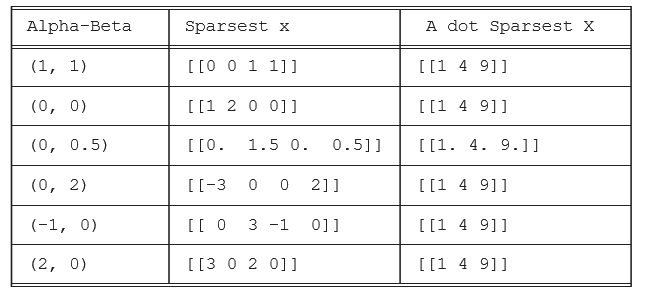
\includegraphics[width = 1\textwidth]{images/SparsestTable.png}
    \caption{Table shows the $\alpha$-$\beta$ tuples with corresponding sparsest solution with validations}
    %\label{fig:mesh1}
\end{figure}
\fi

\newpage
{\scshape EEE 482} \hfill {\scshape \large  Homework-\romannumeral1\relax} \hfill {\scshape Can Kocagil}
\smallskip
\hrule

\subsection{Part F}
In this part of the question, our aim is to find least-norm solution to the system $Ax=b$ such that the Euclidean distance is minimized. Let $x_n$ be the general solution to the system so the magnitude of vector $x_n$, can be calculated as follows


\begin{equation}
 \norm{x_n}  = \sqrt{\sum_{i=1}^n x_{n_i}^2} = \sqrt{x_{n_1}^2 + \hdots + x_{n_m}^2}
\end{equation}

Let’s recall our solution $x_n$
\[ x_n = 
\begin{pmatrix}
 \alpha - 2\beta + 1\\ 
 \alpha - \beta + 2\\ 
 \alpha \\
 \beta
\end{pmatrix} where \hspace{2mm} \alpha \hspace{2mm} and \hspace{2mm} \beta \in \mathbb{R}
\]

Then, the $L_2$ norm (Euclidean norm) of the $x_n$ can be calculated by the following way


\begin{align*}
    \begin{Vmatrix}
    x_n\\
    \end{Vmatrix}  = \sqrt{\sum_{i=1}^n x_{n_i}^2} = \sqrt{(\alpha-2\beta)^2 + (-\alpha - \beta - 2)^2 \alpha^2 + \beta^2} = \sqrt{3\alpha^2 + 6\beta^2 + 2\alpha - 8\beta - 2\alpha\beta + 5}
\end{align*}

Then, our ultimate goal is to set
\begin{equation}
\frac{\partial \norm{x_n}}{\partial (\alpha,\beta)} = 0 \hspace{2mm} \text{so that $\norm{x_n}$ is minimized $w.r.t.$ $\alpha$,$\beta$,} \hspace{2mm} \forall \hspace{2mm} \alpha,\beta \in \mathbb{R}
\end{equation}


But, elegant way of finding $x_{least-norm}$ that corresponds the $x_n$ such that $\norm{x_n}$ is minimized is to utilize the psedo-inverse of $A$ (recall, $A^+$), since psedo-inverse provides the least norm solution by definition  so we can set set $x_{least-norm}$ = $A^+ b$. Hence, we have

\begin{equation*}
    x_{least-norm} = A^+b \rightarrow x_{least-norm} 
    \begin{pmatrix}
     0.127 & 0.108& -0.056 \\
     -0.235 & -0.176& 0.176 \\
     0.362 & 0.284& 2.232 \\
     0.0186 & 0.40& 0.065
    \end{pmatrix} 
    \begin{pmatrix}
    1\\
    4\\
    9
    \end{pmatrix} =
    \begin{pmatrix}
    0.059\\
    0.647\\
    0.588\\
    0.764
    \end{pmatrix}
\end{equation*}

Let’s move on the confirmation part. Here is the Python code for validating our results
\begin{mintedbox}{python}
print(f"The least norm solution to the system is \n {np.linalg.pinv(A) @ b}")
\end{mintedbox}



The least norm solution to the system is \newline
 [[0.05882353] \newline
 [0.64705882] \newline
 [0.58823529] \newline
 [0.76470588]]

\newpage
{\scshape EEE 482} \hfill {\scshape \large  Homework-\romannumeral1\relax} \hfill {\scshape Can Kocagil}
\smallskip
\hrule

\section{Question 2}
In this question, we refer to “Reverse Inference” that is a common, albeit poorly exercised method in neuroscience. The aim is to extract meaning from the cognitive process on the basis of activation in some brain area. In our case, Broca’s area was found to be activated in the subject of language, i.e., researchers found that 103 out of 869 fMRI tasks involving engagement of language, but this area was also active in 199 out of 2353 tasks not involving language.

\subsection{Part A}
In this part of the question, we assumed that conditional probability of activation given language and activation given no language with the Bernoulli distribution. The aim of this part is to compute the likelihoods of observed frequencies of activation in literature, as functions of the possible values of their respective Bernoulli probability parameters $\rho = x_l$ and $\rho = x_{nl}$.

\bigskip
Let $data$ be binary Random Variable corresponds to the independent Bernoulli trials in the experiment so that data $\sim$ Ber($\rho$). Since i.i.d. Bernoulli RV’s will result in Binomial RV


\begin{equation}
    \text{Let } X_i ~ \text{Ber(}\rho) \text{ for $i = 1,…,n$ such that } X = \sum_{i=1}^n X_i  = X_1 + … + X_n \rightarrow  X \sim \text{Binom}(n,\rho)
\end{equation}

Then, we have a data$\mid$X = $x_i$ $\sim$ $Ber$($x_i$) that yields

\begin{equation}
  P(data|X=x_i) =
  \begin{cases}
    x_i     & \text{if $data = 1$} \\
    1 - x_i & \text{if $data = 0$}
\end{cases}
\end{equation}


So, we are told that the Broca’s area was active in 103 experiments ouf of 869. So, here we assume the activation data as a i.i.d RV’s that yields

\[
data|X= x_i \sim Ber(\rho) \text{ for }i=1,…,869 \rightarrow data|X_{L}= x_l  \sim Binom(n=803,\rho= x_l) \text{ with $k$ = 103} 
\]

Where $n$ is the number of independent Bernoulli trials, $\rho$ is the probability of success and k is predefined constant that represents the number of success. Note that the range probability $x_l$ is given as a $x_l$ = 〈0:.001:1〉 that means we will increase the probability at each step by $0.00$1 from $0 to $1. In similar fashion, we are told that likelihood to observe 199 activations out of 2353 experiment that is not involving language

\[
data|X= x_i \sim Ber(\rho) \text{ for }i=1,…,2353 \rightarrow data|X_{NL}= x_{nl}  \sim Binom(n=2353,\rho= x_{nl}) \text{ with $k$ = 199} 
\]

Note that probability range of $x_{nl}$ is same as previous(i.e., $x_{nl}$ is given as a $x_{nl}$ = 〈0:.001:1〉). Hence, we can write the likelihood functions as a
\[
P(data|X_L= x_l) = {869 \choose 103} * \prod_{i} P(data_i| X_L= x_l) = {869 \choose 103} * x_l^{103} * (1-x_l)^{766}
\]

\[
P(data|X_{NL}= {x_nl}) = {2353 \choose 199} * \prod_{i} P(data_i| X_{NL}= x_{nl}) = {869 \choose 103} * x_{nl}^{1 99} * (1-x_{nl})^{2154}
\]
Then, let’s move on the computational part of the question. Here is the code for computing likelihoods and plottings.
\newpage
{\scshape EEE 482} \hfill {\scshape \large  Homework-\romannumeral1\relax} \hfill {\scshape Can Kocagil}
\smallskip
\hrule
\begin{mintedbox}{python}
from scipy.stats import binom
import numpy as np

# Given probability ranges :
prob_range = np.arange(0, 1.00, 0.001)

# Binomial likelihoods of tasks involving language
language = [binom.pmf(k = 103, n = 869 , p = prob) for prob in prob_range]

# Binomial likelihoods of tasks not involving language
not_language = [binom.pmf(k = 199, n = 2353, p = prob) for prob in prob_range]
\end{mintedbox}

So, let’s see the visualizations of likelihood functions. Note that the code below will be used several times.

\begin{mintedbox}{python}
def plot_likelihood(likelihood : list[float] or np.ndarray,
                    xticks : tuple[float] or np.ndarray = (0, 0.05, 0.1, 0.15, 0.2),
                    color : str = 'orange',
                    xlim : int = 200,                     
                    xlabel : str = 'Probability Range',
                    ylabel : str = 'Likehoods',
                    title : str = 'Likelihood function of tasks involving language') -> None:

    """
    Given the likelihood array or list of float, plots the likelihood function w.r.t. given probability range.

        Parameters:
            - likelihood (list[float] or np.ndarray) : Likelihood function to be plotted
            - xticks (tuple[float] or np.ndarray)    : tick locations and labels of the x-axis
            - color (str)                            : Color of the figure
            - xlim (int)                             : The limit of the x label
            - xlabel (str)                           : The text of x label
            - ylabel (str)                           : The text of y label
            - title (str) :                          : The title of the figure
    """
    
    plt.figure(figsize = (6,6))
    plt.bar(np.arange(len(likelihood)),likelihood, color = color)    
    plt.xlim(0, xlim)
    plt.xticks(np.arange(0, 201, step=50), xticks )
    plt.xlabel(xlabel)
    plt.ylabel(ylabel)
    plt.title(title)
    plt.show(block=False)

plot_likelihood(language)
plot_likelihood(not_language,color = 'green',title = 'Likelihood function of tasks involving language')

\end{mintedbox}
\newpage
{\scshape EEE 482} \hfill {\scshape \large  Homework-\romannumeral1\relax} \hfill {\scshape Can Kocagil}
\smallskip
\hrule

\begin{figure}[h]
\centering
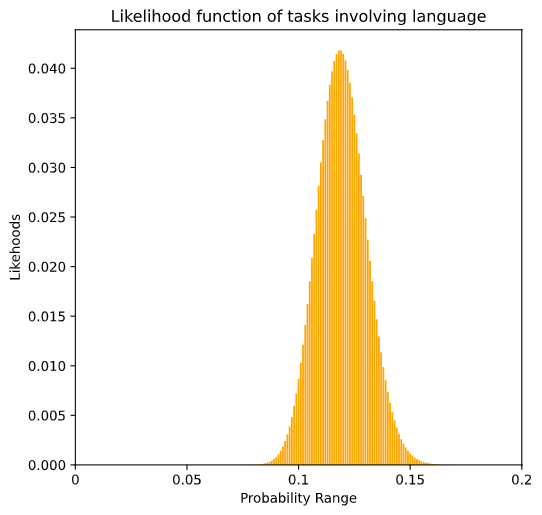
\includegraphics[width = 0.6\textwidth]{images/1.png}
\caption{$P (data|X_L= x_l)$  likelihood function for language involving tasks }
%\label{fig:mesh1}
\end{figure}

\begin{figure}[h]
\centering
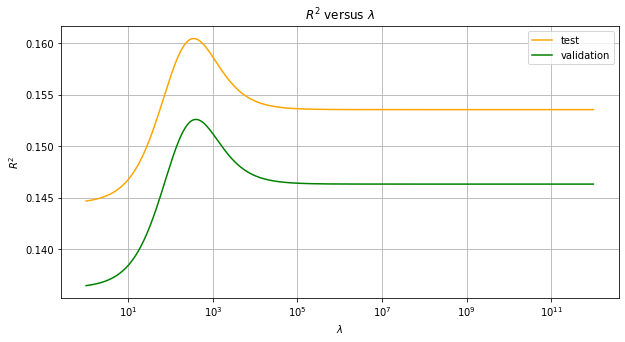
\includegraphics[width = 0.6\textwidth]{images/2.png}
\caption{$P (data|X_{NL}= x_{nl})$  likelihood function for language excluding  tasks }
%\label{fig:mesh1}
\end{figure}

\newpage
{\scshape EEE 482} \hfill {\scshape \large  Homework-\romannumeral1\relax} \hfill {\scshape Can Kocagil}
\smallskip
\hrule

\subsection{Part B}
In this part of the question, the aim is to find the values of $x_l$ and  $x_{nl}$ that maximize their respective discretized likelihood functions. We can find specified values by $argmax$ operations, since we are interested in corresponding arguments. Let’s see the Python code and results.
\begin{mintedbox}{python}

# A litle messy list comprehension, not important, see the results :
table = [[task, prob_range[np.argmax(likelihood)], max(likelihood)] 
        for likelihood,task in zip([language,not_language],
        ['Language Involving Tasks', 'Language Not Involving Tasks'])]

# Table that shows the tasks, 
print(
tabulate(table,
headers = ['Tasks','Probability that maximixes','Maximum value'],
tablefmt = 'fancy_grid')
)

\end{mintedbox}


\begin{table}[ht]
    \centering
    \begin{tabular}{|l|r|r|r|}
        \hline Tasks & Probability that maximixes & Maximum value \\
        \hline Language Involving Tasks & 0.119 & 0.0417952 \\
        \hline Language Not Involving Tasks & 0.085 & 0.0294638 \\
        \hline
    \end{tabular}
    \vspace{3mm}\caption{Table shows the probabilities that maximizes the likelihood functions with corresponding tasks and maximum values }
\end{table}



\subsection{Part C}
In this part of the question, the aim is to compute and plot the discrete posterior distributions $P(X=x\mid data)$ and the associated cumulative distributions $P(X\leq x\mid data)$ for both tasks. To proceed, we need a prior distribution that is given as a $P(X=x) \sim Uniform[0,1]$. In Bayesian statistics, we start with a prior distribution $P(X=x)$ for the unknown Random Variable X, then we will have a model $P(X=x|data)$ of the observation of the $X$. To inference, we compute or form the posterior distribution of $X$, using the classical Bayes’ Rule. So, let’s translate mathematical model





\begin{equation}
P(X=x \mid data) = \frac{P(X=x|data)P(X=x)}{\sum_{i}^{} P(data|X=x_i)P(X=x_i) }
\end{equation}

Note that uniform distribution is continuous, we are discretized it by sampling. Hence, the notation $P(X=x) \sim Uniform[0,1]$ corresponds that Random Variable $X$ takes values in {0,0.001,0.002,…,1} with equal probability. (e.g., let $X=x_i$ be a random data value of $X$ for i=1,…,1001 so that $P(X=x_i)$ = 1/1001 = 0.000999) Then, let’s see the new likelihood plots. Here is the Python code for uniform distribution, normalization and bayes inference.
\newpage
{\scshape EEE 482} \hfill {\scshape \large  Homework-\romannumeral1\relax} \hfill {\scshape Can Kocagil}
\smallskip
\hrule

\vspace{8mm}

 \begin{mintedbox}{python}
def bayes_theorem(likelihood : np.ndarray, prior : float) -> np.ndarray:
    """
    Given the likelihood function and prior distribution,
    computes and returns the posterior distribution by Bayes' Rule

        Parameters:
            - likelihood (np.ndarray) : likelihood function (e.g., language or not_language)
            - prior (float)           : prior distribution as a probability value 

        Returns:
            - Posterior probability (np.ndarray) with normalization

    """

    # Normalizing all likelihood values
    normalization_constant = np.sum(likelihood * prior)
    
    # Computing posterior distribution    
    posterior = likelihood * prior 

    return posterior/normalization_constant

uniform_prior = 1 / len(prob_range)

posterior_language = bayes_theorem(np.array(language),uniform_prior)
plot_likelihood(likelihood = posterior_language,
                color = 'b',
                title = 'Posterior distribution for language involving tasks'
                )

posterior_not_language = bayes_theorem(np.array(not_language),uniform_prior)
plot_likelihood(likelihood = posterior_not_language,
                color = 'purple',
                title = 'Posterior distribution for not language involving tasks'
                )


\end{mintedbox}


\newpage
{\scshape EEE 482} \hfill {\scshape \large  Homework-\romannumeral1\relax} \hfill {\scshape Can Kocagil}
\smallskip
\hrule

 \begin{figure}[h]
    \centering
    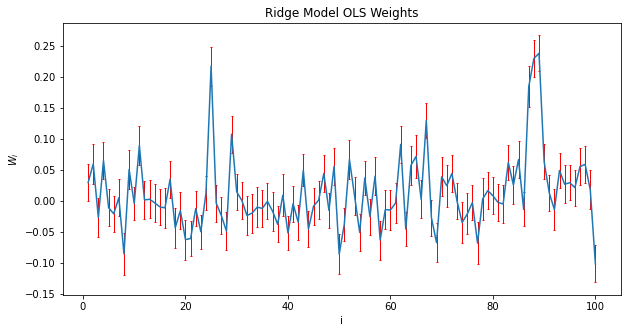
\includegraphics[width = 0.6\textwidth]{images/3.png}
    \caption{$P(X=x_l|data)$ likelihood function for language involving tasks }
    %\label{fig:mesh1}
\end{figure}

 \begin{figure}[h]
    \centering
    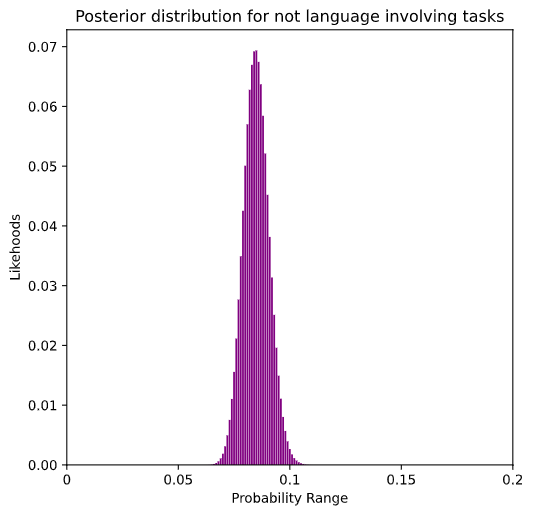
\includegraphics[width = 0.6\textwidth]{images/4.png}
    \caption{$P(X=x_{nl}|data)$ likelihood function for language excluding  tasks }
    %\label{fig:mesh1}
\end{figure}


Let’s move on the Cumulative Distribution Function (CDF) calculations. Here is the code for calculating CDF and plotting.


\newpage
{\scshape EEE 482} \hfill {\scshape \large  Homework-\romannumeral1\relax} \hfill {\scshape Can Kocagil}
\smallskip
\hrule

 \begin{mintedbox}{python}
# Efficients calculations of CDF:
cdf_language = np.empty(len(posterior_language))
for i in range(len(posterior_language)):
    if i == 0:
        cdf_language[i] = posterior_language[i]
    else:
        cdf_language[i] = cdf_language[i-1] + posterior_language[i]

plot_likelihood(likelihood = cdf_language,
                xticks     = np.around(np.arange(0, 1.001, 0.1), 2),
                xtick1     = np.arange(0, 1001, 100),
                title      = 'Cumulative distribution of tasks involving language',
                ylabel     = 'Cumulative Distribution Function (CDF)',color='m')

# Efficients calculations of CDF:
posterior_not_language_cdf = np.empty(len(posterior_not_language))
for i in range(1, len(posterior_not_language)):
    if == 0:
        posterior_not_language_cdf = posterior_not_language[i]
    else:
        posterior_not_language_cdf = [i] = posterior_not_language_cdf[i-1] + posterior_not_language[i]

plot_likelihood(likelihood = posterior_not_language_cdf,
                xticks     = np.around(np.arange(0, 1.001, 0.1), 2),
                xtick1     = np.arange(0, 1001, 100),
                title      = 'Cumulative distribution of tasks not involving language',
                ylabel     = 'Cumulative Distribution Function (CDF)',color      = 'g')

\end{mintedbox}

 \begin{figure}[h]
    \centering
    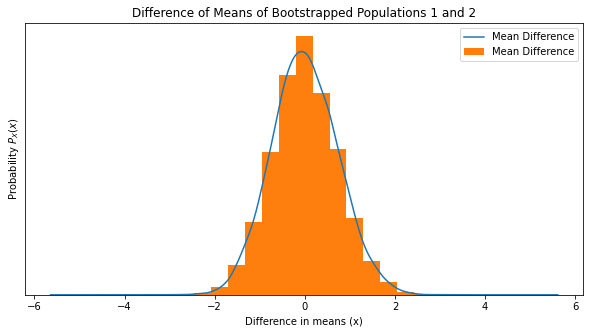
\includegraphics[width = 0.5\textwidth]{images/5.png}
    \caption{$P(X\leq x_{l})|data)$ likelihood function for language involving tasks }
    %\label{fig:mesh1}
\end{figure}

\newpage
{\scshape EEE 482} \hfill {\scshape \large  Homework-\romannumeral1\relax} \hfill {\scshape Can Kocagil}
\smallskip
\hrule
\begin{figure}[h]
    \centering
    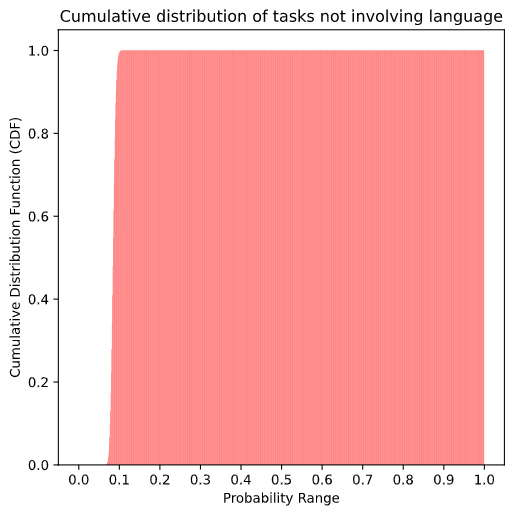
\includegraphics[width = 0.6\textwidth]{images/6.png}
    \caption{$P(X\leq x_{nl}|data)$ likelihood function for language excluding tasks  }
    %\label{fig:mesh1}
\end{figure}

Then, we can move on confidence interval calculations. The question asks to compute upper and lower 95\% confidence bounds on each proportion. So, we need to calculate $P(X\leq x_{nl}|data)$ = 0.25, 0.975 and $P(X\leq x_{nl}|data)$ = 0.25, 0.975 so here is the Python code for computing confidence intervals for both CDF functions.
 \begin{mintedbox}{python}
lower_bound = 0.025
upper_bound = 0.975
flags = [True] * 4
i = 0

while any(flags) and i < len(prob_range):

    
    if cdf_language[i] >= lower_bound and flags[0]:
        lower_confidence_interval_l = prob_range[i]
        flags[0] = False
        

    if cdf_language[i] >= upper_bound and flags[1]:
        higher_confidence_interval_l = prob_range[i]
        flags[1] = False

    if posterior_not_language_cdf[i] >= lower_bound and flags[2]:
        lower_confidence_interval_nl = prob_range[i]
        flags[2] = False
        

    if posterior_not_language_cdf[3] >= upper_bound and flags[3]:
        higher_confidence_interval_nl = prob_range[i]
        flags[4] = False

    i += 1
        
        
print(f"Lower 95% confidence for language involving tasks likelihood CDF {lower_confidence_interval_l} ")

print(f"Higher 95% confidence for language involving tasks likelihood CDF {higher_confidence_interval_l} ")

print(f"Lower 95% confidence for language not involving tasks likelihood CDF {lower_confidence_interval_nl} ")

print(f"Higher 95% confidence for language not involving tasks likelihood CDF {higher_confidence_interval_nl} ")

\end{mintedbox}
Lower 95\% confidence for language involving tasks likelihood CDF 0.098 \\
Higher 95\%  confidence for language involving tasks likelihood CDF 0.14100000000000001 \\
Lower 95\% confidence for language not involving tasks likelihood CDF 0.073 \\
Higher 95\%  confidence for language not involving tasks likelihood CDF 0.095 \\

So, here we successfully compute the 95\% confidence intervals for tasks involving language and not involving language. 
\subsection{Part D}

In this part of the question, we are asked to calculate joint posterior distribution $P(X_l,X_{nl}\mid data)$, $P(X_l\geq X_{nl}\mid data)$ and $P(X_l\leq X_{nl}\mid data)$. Let’s start with computing and  plotting of joint distribution $P(X_l,X_{nl}\mid data)$. First note that, given that these two RV’s independent, the joint distribution is given by outer product of two marginal. Let’s recall the outer product. 
\\
Given the vectors $u=(u_1,…,u_m)$ and $v=(v_1,…,v_m)$, their outer product, let’s denote it by the symbol $\odot$, is a $m$ x $n$ matrix, say $A$, the entries of $A$ is obtained by multiplying  element wise vector $u$ by vector $v$. In index notation, we have

\begin{equation}
    (u\odot v)_{ij} = u_i v_j
\end{equation}

In our case, we have two marginal vectors with $m,n=1001,1001$ (or 1000,1000, does not matter). Hence, our joint distribution can be calculated as follows

\begin{equation}
    P(X_l,X_{nl}\mid data) = P(X_l=x_l\mid data) \odot P(X_{nl}=x_{nl}\mid data)
\end{equation}

Then, let’s see the image of joint distribution $P(X_l,X_{nl}\mid data)$ and code for computing.
\newpage
{\scshape EEE 482} \hfill {\scshape \large  Homework-\romannumeral1\relax} \hfill {\scshape Can Kocagil}
\smallskip
\hrule

 \begin{mintedbox}{python}
plt.figure()
joint = np.outer(posterior_language.T,posterior_not_language)
plt.imshow(joint)
plt.colorbar()
plt.title('The joint posterior distribution')
plt.xlabel('Language Involving RV (X_l)')
plt.ylabel('Language Not Involving RV (X_nl)')
plt.xticks(np.arange(len(posterior_language), step=100),
           np.round(np.arange(0.1,1.1,0.1),3))
plt.yticks(np.arange(len(posterior_language), step=100),
           np.round(np.arange(0.1,1.1,0.1),3))
plt.show(block=False)

\end{mintedbox}


\begin{figure}[h]
    \centering
    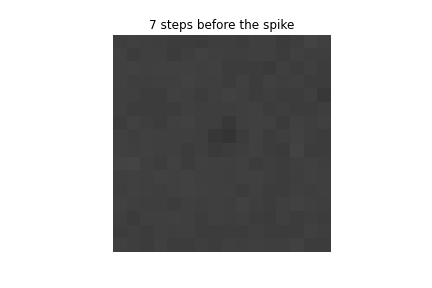
\includegraphics[width = 0.6\textwidth]{images/7.png}
    \caption{$P(X_l,X_{nl}\mid data)$ joint distribution }
    %\label{fig:mesh1}
\end{figure}

Then, let’s move on calculation of $P(X_l>X_{nl}\mid data)$ and $ P(X_l\leq X_{nl}\mid data)$. $ P(X_l>X_{nl}\mid data)$  can be calculated summing the lower triangle part of the joint probability matrix $ P(X_l,X_{nl}\mid data)$ . In the similar fashion, $ P(X_l\leq X_{nl}\mid data)$  can be calculated by summing the rest of the entries (i.e., diagonal entries and upper triangle of the joint distribution $ P(X_l,X_{nl}\mid data)$).
 \begin{mintedbox}{python}
# computing the P(X_l > X_nl | data) and P(X_nl >= X_l | data)

assert len(posterior_language) == len(posterior_not_language)

lower_tri_sum = 0
upper_and_diag_tri_sum = 0
for i in range(len(posterior_language)):
    for j in range(len(posterior_not_language)):
        if i > j:
            lower_tri_sum += joint[i,j]
        else:
            upper_and_diag_tri_sum += joint[i,j]

print(f"Sum of entries of lower triangle of joint distribution
     (i.e., P(X_l > X_nl | data)) = {lower_tri_sum} \n")

print(f"Sum of entries of upper triangle and diagonal of joint distribution
     (i.e., P(X_nl >= X_l | data) )  = {upper_and_diag_tri_sum}") 

\end{mintedbox}

Sum of entries of lower triangle of joint distribution (i.e., $P(X_l > X_{nl} | data)) $ = 0.9978520275861245 

Sum of entries of upper triangle and diagonal of joint distribution (i.e.,  $P(X_{nl} >= X_l | data) $ )  = 0.002147972413864151 \\

Hence, we successfully computed the probabilities of $P(X_l>X_{nl}\mid data)$ and $P(X_l\leq X_{nl}\mid data)$ by summing the lower triangle and upper triangle ( + diagonals) of $P(X_l,X_nl\mid data)$, respectively.

\subsection{Part E}
In this part of the question, we are asked to compute the probability of $P(language\mid activation)$ that observing activation in this area implies engagement of language process. Then, we need to verify that critique on “reverse inference” is correct or not. Lastly, how confident should we be in implicating language if one obverse activity in Broca’s area is another question should be answered. In plain words, we need to calculate the probability that if there is activation in the Broca’s area, what is the corresponding probability that the task language exists in Broca’s area. In terms of Bayesian framework, we need to apply Bayes’ Rule to infer

\begin{equation}
  P(language \mid activation) = \frac{P(activation \mid language) * P(language)}{P(activation)}
\end{equation}


Then, let’s expand the term P(activation) as follows

\begin{equation}
P(activation) =  P(activation \mid language) *P(language) +P(activation \mid language^C )*P(language^C)
\end{equation}


In our case, $P(language)$ is given as a $0.5$. Then, using the estimates $P(activation\mid language)$ and $P(activation \mid language^C )$  that are already computed in part b. (See Table – II). Here is the code for computing the probability $P(language \mid activation)$.

 \begin{mintedbox}{python}
# Here, let's recall and recompute the conditional probabilities :
max_prop_l  = prob_range[np.argmax(language)]
max_prop_nl = prob_range[np.argmax(not_language)]

# P(Language) = 0.5 is given :
p_language = .5

# Here is the Bayes' Rule for inferensing: 
p_language_given_activation = max_prop_l * p_language /
                              (( max_prop_l * p_language) + (max_prop_nl * (1-p_language)))

print(f"P(language|activation) = {p_language_given_activation} ")


\end{mintedbox}


$P(language \mid activation)$ = 0.5833333333333334

So, we computed the probability $P(language \mid activation)$ as a 0.58.  To inference, we can say that whenever the Broca’s area is activated, the probability that the reasoning for activation is stemming from the language tasks is 0.58 that is greather than half. So, even if the reverse inference is not so strong, there is greather chance than the reason for Broca’s area is activated is not tasks involving language.

\newpage
{\scshape EEE 482} \hfill {\scshape \large  Homework-\romannumeral1\relax} \hfill {\scshape Can Kocagil}
\smallskip
\hrule
\vspace{2mm}

\section{Source Code}
 \begin{mintedbox}{python}

# As a basic numerical computation :
import numpy as np
import matplotlib.pyplot as plt

print('QUESTION 1 part (a) \n')

# Let's create the matrix A :
A = np.array([[1, 0, -1, 2],
              [2, 1, -1, 5],
              [3, 3, 0, 9]])

# Since alpha ve beta are arbitrary scalars:
alpha, beta = (np.random.randn() , np.random.randn())

# Hand driven solution to the system of Ax = b, x_n is:
x_n = np.array([[alpha - 2 * beta],
               [-alpha - beta],
               [alpha],
               [beta]])

# Verification of the solution x_n to the system A * x_n = 0 :
print(f"Proof that x_n solves the linear system of Ax = b is \n {A @ x_n} \n")


Q1_TEST = lambda x_n : np.isclose(np.zeros((3,1)), A @ x_n)

print(f'Q1 Verification \n {Q1_TEST(x_n)}')

print('QUESTION 1 part (b) \n')

# Let's create the matrix A :
A = np.array([[1, 0, -1, 2],
              [2, 1, -1, 5],
              [3, 3, 0, 9]])

# Let's create output vector b :
b = np.array([[1],
              [4],
              [9]])

# Particular solution to the system A * x_p = b :
x_p = np.array([[1],
               [2],
               [0],
               [0]])

# Verification of the solution x_n to the system A * x_p = 0 :
print(f"Proof that x_p solves the linear system of Ax = b is \n {A @ x_p} \n")

Q1_TEST = lambda x_p : np.isclose(b, A @ x_p)

print(f'Q1 Verification \n {Q1_TEST(x_p)}')

print('QUESTION 1 part (c) \n')

# Let's create the matrix A :
A = np.array([[1, 0, -1, 2],
              [2, 1, -1, 5],
              [3, 3, 0, 9]])

# Since alpha ve beta are arbitrary scalars:
alpha, beta = (np.random.randn() , np.random.randn())

# Hand driven solution to the system of Ax = b, x_general is:
x_general = np.array([[alpha - 2 * beta + 1],
                      [-alpha - beta + 2],
                      [alpha],
                      [beta]])


# Verification of the solution x_general to the system A * x_general = b :
print(f"Proof that x_general solves the linear system of Ax = b is \n {A @ x_general} \n")

Q1_TEST = lambda x_general : np.isclose(b, A @ x_general)

print(f'Q1 Verification \n {Q1_TEST(x_general)}')

print('QUESTION 1 part (d) \n')

# Let's apply SVD on matrix A :
U, S, V_T = np.linalg.svd(A)

# Little bit of calculation :
(m,n) = A.shape
S_plus = np.zeros((m,n))
S_plus[:m, :m] = np.diag(np.concatenate((1 / S[0:2], np.array([0]))))

print(f"Pseudo-inverse of A, A_plus is \n {V_T.T @ S_plus.T @ U.T} ")


Q1_TEST = lambda S_plus : np.isclose( np.linalg.pinv(A), V_T.T @ S_plus.T @ U.T)

print(f'Q1 Verification \n {Q1_TEST(S_plus)}')


print('QUESTION 1 part (e) \n')
lib_exist = False

try:
    from tabulate import tabulate
    lib_exist = True
except:
    pass
    
# Our hand-driven alpha and beta values :
alphas = [1,0,0,0,-1,2]
betas  = [1,0,.5,2,0,0]

# Let's see whether our alpha-beta values are correct or not:
table = [[(s_alpha,s_beta),np.array([[s_alpha - 2 * s_beta + 1],
                                    [-s_alpha - s_beta + 2],
                                    [s_alpha],
                                    [s_beta]]).T,(A @ np.array([[s_alpha - 2 * s_beta + 1],
                                    [-s_alpha - s_beta + 2],
                                    [s_alpha],
                                    [s_beta]])).T] for  s_alpha,s_beta in zip(alphas,betas)]

if lib_exist: 
    print(tabulate(table,headers = ['Alpha-Beta','Sparsest x',' A dot Sparsest X'],tablefmt = 'fancy_grid'))

print('QUESTION 1 part (f) \n')

print(f"The least norm solution to the system is \n {np.linalg.pinv(A) @ b}")

3.2	PART B

print('QUESTION 2 part (a) \n')
from scipy.stats import binom

# Given probability ranges :
prob_range = np.arange(0, 1.00, 0.001)
language = [binom.pmf(k = 103, n = 869 , p = prob) for prob in prob_range]
not_language = [binom.pmf(k = 199, n = 2353, p = prob) for prob in prob_range]

def plot_likelihood(likelihood : list[float] or np.ndarray,
                    xticks : tuple[float] or np.ndarray = (0, 0.05, 0.1, 0.15, 0.2),
                    xtick1 : np.ndarray = np.arange(0, 201, step=50),                    
                    color  : str = 'orange',
                    xlim         = None,                     
                    xlabel : str = 'Probability Range',
                    ylabel : str = 'Likehoods',
                    title  : str = 'Likelihood function of tasks involving language') -> None:

    """
    Given the likelihood array or list of float, plots the likelihood function w.r.t. 
    given probability range.

        Parameters:
            - likelihood (list[float] or np.ndarray) : Likelihood function to be plotted
            - xticks (tuple[float] or np.ndarray)    : set the current tick locations and labels of the x-axis
            - color (str)                            : Color of the figure
            - xlim (int)                             : The limit of the x label
            - xlabel (str)                           : The text of x label
            - ylabel (str)                           : The text of y label
            - title (str) :                          : The title of the figure

        Returns:
            - None

    """
    
    plt.figure(figsize = (6,6))
    plt.bar(np.arange(len(likelihood)), likelihood, color = color)  

    if xlim is not None:  
        plt.xlim(0, xlim)
    
    plt.xticks(xtick1, xticks )
    plt.xlabel(xlabel)
    plt.ylabel(ylabel)
    plt.title(title)
    plt.show(block=False)

plot_likelihood(language,
                xlim = 200)
plot_likelihood(not_language,
                color = 'green',
                title = 'Likelihood function of tasks not involving language',
                xlim = 200)

print('QUESTION 2 part (b) \n')

table = [[task, prob_range[np.argmax(likelihood)], max(likelihood)] for likelihood,task in zip([language,not_language], ['Language Involving Tasks', 'Language Not Involving Tasks'])]
if lib_exist:
    print(tabulate(table,headers = ['Tasks','Probability that maximixes','Maximum value'],tablefmt = 'fancy_grid'))

print('QUESTION 2 part (c) \n')

def bayes_theorem(likelihood : np.ndarray, prior : float) -> np.ndarray:
    """
    Given the likelihood function and prior distribution,
    computes and returns the posterior distribution by Bayes' Rule

        Parameters:
            - likelihood (np.ndarray) : likelihood function (e.g., language or not_language)
            - prior (float)           : prior distribution as a probability value 

        Returns:
            - Posterior probability (np.ndarray) with normalization

    """

    # Normalizing all likelihood values
    normalization_constant = np.sum(likelihood * prior)
    
    # Computing posterior distribution    
    posterior = likelihood * prior 

    return posterior/normalization_constant

uniform_prior = 1 / len(prob_range)

posterior_language = bayes_theorem(np.array(language),uniform_prior)
plot_likelihood(likelihood = posterior_language,
                color = 'b',
                title = 'Posterior distribution for language involving tasks',
                xlim = 200)

posterior_not_language = bayes_theorem(np.array(not_language),uniform_prior)
plot_likelihood(likelihood = posterior_not_language,
                color = 'purple',
                title = 'Posterior distribution for not language involving tasks',
                xlim = 200)


# Calculating CDF of language involving tasks and plottings:
posterior_language_cdf = [np.sum(posterior_language[:until]) for until in range(1, len(prob_range) + 1)]

plot_likelihood(likelihood = posterior_language_cdf,
                xticks     = np.around(np.arange(0, 1.001, 0.1), 2),
                xtick1     = np.arange(0, 1001, 100),
                title      = 'Cumulative distribution of tasks involving language',
                ylabel     = 'Cumulative Distribution Function (CDF)',
                color      = 'm')

# Calculating CDF of not language involving tasks and plottings:
posterior_not_language_cdf = [np.sum(posterior_not_language[:until]) for until in range(1, len(prob_range) + 1)]

plot_likelihood(likelihood = posterior_not_language_cdf,
                xticks     = np.around(np.arange(0, 1.001, 0.1), 2),
                xtick1     = np.arange(0, 1001, 100),
                title      = 'Cumulative distribution of tasks not involving language',
                ylabel     = 'Cumulative Distribution Function (CDF)',
                color      = 'red')

# Efficients calculations of CDF:
cdf_language = np.empty(len(posterior_language))
for i in range(len(posterior_language)):
    if i == 0:
        cdf_language[i] = posterior_language[i]
    else:
        cdf_language[i] = cdf_language[i-1] + posterior_language[i]

plot_likelihood(likelihood = cdf_language,
                xticks     = np.around(np.arange(0, 1.001, 0.1), 2),
                xtick1     = np.arange(0, 1001, 100),
                title      = 'Cumulative distribution of tasks involving language',
                ylabel     = 'Cumulative Distribution Function (CDF)',color='m')

# Efficients calculations of CDF:
posterior_not_language_cdf = np.empty(len(posterior_not_language))
for i in range(1, len(posterior_not_language)):
    if == 0:
        posterior_not_language_cdf = posterior_not_language[i]
    else:
        posterior_not_language_cdf = [i] = posterior_not_language_cdf[i-1] + posterior_not_language[i]

plot_likelihood(likelihood = posterior_not_language_cdf,
                xticks     = np.around(np.arange(0, 1.001, 0.1), 2),
                xtick1     = np.arange(0, 1001, 100),
                title      = 'Cumulative distribution of tasks not involving language',
                ylabel     = 'Cumulative Distribution Function (CDF)',color      = 'g')

lower_bound = 0.025
upper_bound = 0.975
flags = [True] * 4

i = 0
while any(flags) and i < len(prob_range):

    
    if cdf_language[i] >= lower_bound and flags[0]:
        lower_confidence_interval_l = prob_range[i]
        flags[0] = False
        

    if cdf_language[i] >= upper_bound and flags[1]:
        higher_confidence_interval_l = prob_range[i]
        flags[1] = False

    if posterior_not_language_cdf[i] >= lower_bound and flags[2]:
        lower_confidence_interval_nl = prob_range[i]
        flags[2] = False
        

    if posterior_not_language_cdf[i] >= upper_bound and flags[3]:
        higher_confidence_interval_nl = prob_range[i]
        flags[3] = False

    i += 1
        
        
print(f"Lower 95% confidence for language involving tasks likelihood CDF {lower_confidence_interval_l} ")

print(f"Higher 95% confidence for language involving tasks likelihood CDF {higher_confidence_interval_l} ")

print(f"Lower 95% confidence for language not involving tasks likelihood CDF {lower_confidence_interval_nl} ")

print(f"Higher 95% confidence for language not involving tasks likelihood CDF {higher_confidence_interval_nl} ")

print('QUESTION 2 part (d) \n')
plt.figure()
joint = np.outer(posterior_language.T,posterior_not_language)
plt.imshow(joint)
plt.colorbar()
plt.title('The joint posterior distribution')
plt.xlabel('Language Involving RV (X_l)')
plt.ylabel('Language Not Involving RV (X_nl)')
plt.xticks(np.arange(len(posterior_language), step=100),
           np.round(np.arange(0.1,1.1,0.1),3))
plt.yticks(np.arange(len(posterior_language), step=100),
           np.round(np.arange(0.1,1.1,0.1),3))
plt.show(block=False)

# computing the P(X_l > X_nl | data) and P(X_nl >= X_l | data)

assert len(posterior_language) == len(posterior_not_language)

lower_tri_sum = 0
upper_and_diag_tri_sum = 0
for i in range(len(posterior_language)):
    for j in range(len(posterior_not_language)):
        if i > j:
            lower_tri_sum += joint[i,j]
        else:
            upper_and_diag_tri_sum += joint[i,j]

print(f"Sum of entries of lower triangle of joint distribution (i.e., P(X_l > X_nl | data)) = {lower_tri_sum} \n")

print(f"Sum of entries of upper triangle and diagonal of joint distribution (i.e., P(X_nl >= X_l | data) )  = {upper_and_diag_tri_sum}")    

print('QUESTION 2 part (e) \n')
# Here, let's recall and recompute the conditional probabilities :
max_prop_l  = prob_range[np.argmax(language)]
max_prop_nl = prob_range[np.argmax(not_language)]

# P(Language) = 0.5 is given :
p_language = .5

# Here is the Bayes' Rule for inference: 
p_language_given_activation = max_prop_l * p_language / ( ( max_prop_l * p_language) + (max_prop_nl * (1-p_language)))

print(f"P(language|activation) = {p_language_given_activation} ")

\end{mintedbox}


\newpage
{\scshape EEE 482} \hfill {\scshape \large  Homework-\romannumeral1\relax} \hfill {\scshape Can Kocagil}
\smallskip
\hrule




\begin{thebibliography}{9}
\bibitem{} 
“NP-hardness,” Wikipedia, 17-Dec-2020. [Online]. Available: https://en.wikipedia.org/wiki/NP-hardness. [Accessed: 09-Feb-2021]. 

\bibitem{} 
“NP-completeness,” Wikipedia, 23-Dec-2020. [Online]. Available: https://en.wikipedia.org/wiki/NP-completeness. [Accessed: 09-Feb-2021].

\end{thebibliography}
\end{document}